\chapter{Antecedentes y estado del arte}
\label{chap:antecedentes}
\mtcsettitle{minitoc}{Contenidos} 
\minitoc
 
 
\section{Resistencia al avance. El problema de la extrapolación modelo--buque}
\label{sec:extrapolacion}

La predicción de la resistencia al avance de un buque a escala buque a partir de ensayos con modelos físicos se basa en la \textbf{similitud dinámica}. Dos flujos alrededor de cuerpos geométricamente semejantes son dinámicamente similares si comparten los mismos grupos adimensionales que gobiernan la física del flujo. Para el caso de un buque de superficie en aguas tranquilas, las ecuaciones de Navier-Stokes adimensionalizadas revelan dos parámetros fundamentales: el \textbf{número de Reynolds} $Re = VL/\nu$, que expresa la relación entre fuerzas inerciales y viscosas, y el \textbf{número de Froude} $Fr = V/\sqrt{gL}$, que expresa la relación entre fuerzas inerciales y gravitatorias. En ambos parámetros, $V$ es la velocidad de avance, $L$ la eslora característica, $\nu$ la viscosidad cinemática del agua y $g$ la aceleración de la gravedad. En esta tesis se adopta $L = L_{OS}$, la eslora total sumergida, para el número de Reynolds, por ser la longitud sobre la que efectivamente se desarrolla la capa límite, y $L = L_{WL}$, la eslora en flotación, para el número de Froude, por ser la que gobierna el tren de olas generado. La similitud dinámica completa requeriría igualdad simultánea de ambos parámetros entre modelo ($M$) y buque ($S$):
%
\begin{equation}
    Re_M = Re_S \qquad \text{y} \qquad Fr_M = Fr_S.
\end{equation}
%
Sin embargo, al utilizar agua en ambas escalas ($\nu_M \approx \nu_S$, $g_M = g_S$), estas dos condiciones imponen escalas de velocidad contradictorias. La igualdad de Froude exige $V_M = V_S / \sqrt{\lambda}$, mientras que la igualdad de Reynolds exige $V_M = V_S \cdot \lambda$, siendo $\lambda = L_S / L_M$ el factor de escala lineal. Para valores típicos de $\lambda$ entre 20 y 80, es imposible satisfacer ambas condiciones simultáneamente con agua como fluido de trabajo \citep{birk2019}.

La solución práctica, establecida históricamente por William Froude, consiste en respetar la similitud de Froude durante los ensayos (capturando correctamente la generación de olas) y corregir analíticamente la diferencia en la componente viscosa. Esta \textbf{similitud dinámica parcial} introduce los denominados ``efectos de escala'': diferencias sistemáticas entre el flujo de modelo y el del buque que no están capturadas por la extrapolación estándar y que constituyen la problemática central de esta tesis.

Para cuantificar la resistencia de manera independiente de la escala, se trabaja con el \textbf{coeficiente adimensional de resistencia total}:
%
\begin{equation}\label{eq:CT}
    C_T = \frac{R_T}{\tfrac{1}{2}\,\rho\,V^2\,S},
\end{equation}
%
donde $R_T$ es la fuerza de resistencia total, $\rho$ la densidad del agua
y $S$ la superficie mojada del casco. De manera
análoga se definen los coeficientes de resistencia viscosa $C_V$, friccional
$C_F$, por presión viscosa $C_{PV}$ y por formación de olas $C_W$, todos
referidos a la misma presión dinámica y superficie mojada. Los subíndices
$M$ y $S$ se utilizan a lo largo de esta tesis para distinguir las
magnitudes correspondientes al modelo y al buque respectivamente.

% ---------------------------------------------------------------------
% [REESCRITO] Planteo explícito de la no similitud: separación Re / Fr,
% hipótesis central de Hughes y forma final de C_TS.
% ---------------------------------------------------------------------
Con esta notación el problema de la no similitud puede plantearse de manera
precisa. El coeficiente de resistencia total es función de los dos parámetros
que gobiernan el flujo, $C_T = C_T(Re, Fr)$. El ensayo entrega un único valor
medido, $C_{TM}$, obtenido a $Fr_M = Fr_S$ pero a $Re_M \ll Re_S$: el punto
ensayado no es el punto que se desea predecir. Sin una hipótesis adicional el
dato experimental es, en rigor, inutilizable, porque nada permite discriminar
qué parte de $C_{TM}$ se modifica al pasar de $Re_M$ a $Re_S$ y qué parte
permanece. La extrapolación solo resulta posible si se postula que $C_T$ admite
una descomposición en dos términos \emph{separables}, uno función exclusiva del
número de Reynolds y otro función exclusiva del número de Froude. La propuesta de
\citet{hughes1954} le da forma concreta a esa separación:
%
\begin{equation}\label{eq:CT_decomposicion_hughes}
    C_T(Re,Fr) = (1+k)\,C_{F0}(Re) + C_W(Fr),
\end{equation}
%
donde $C_W$ es el coeficiente de resistencia por formación de olas, $C_{F0}$ es
el coeficiente de resistencia friccional adimensional de una \emph{placa plana
equivalente} --una placa plana bidimensional de la misma eslora y la misma
superficie mojada que el casco, evaluada al mismo número de Reynolds-- y $(1+k)$
es el \textbf{factor de forma}, un multiplicador de origen puramente geométrico.

El primer término de la Ecuación~\eqref{eq:CT_decomposicion_hughes} es la
resistencia viscosa total del casco,
%
\begin{equation}\label{eq:CV}
    C_V = C_F + C_{PV},
\end{equation}
%
que reúne la fricción $C_F$, integral de los esfuerzos de corte sobre la
superficie mojada, y la resistencia de presión viscosa $C_{PV}$, resultante de la
distribución de presiones que la propia capa límite modifica respecto de la del
flujo no viscoso. Ninguna de las dos existe sobre una placa plana en la misma
forma: el casco es tridimensional y curvo, de modo que su fricción es algo mayor
que la de la placa equivalente y, sobre todo, aparece una componente de presión
que la placa no tiene. La propuesta de Hughes consiste en afirmar que toda esa
diferencia puede absorberse en un único multiplicador geométrico,
%
\begin{equation}\label{eq:hughes}
    C_V = (1+k)\, C_{F0}.
\end{equation}

Los dos términos de la Ecuación~\eqref{eq:CT_decomposicion_hughes} cumplen
papeles opuestos en la extrapolación. El término de olas es el que el ensayo
reproduce correctamente: como el modelo se remolca respetando la semejanza de
Froude, $C_W$ toma el mismo valor en ambas escalas y no requiere corrección
alguna; en contrapartida, no se dispone de una expresión analítica para
calcularlo. El término viscoso es exactamente el complementario: es el que
cambia entre escalas, pero es también el único que la hipótesis permite evaluar
en forma cerrada a cualquier número de Reynolds. El procedimiento se reduce
entonces a tres pasos. Primero, despejar del ensayo aquello que no se sabe
calcular,
%
\begin{equation}\label{eq:cw_despejado}
    C_W(Fr) = C_{TM} - (1+k)\,C_{F0}(Re_M);
\end{equation}
%
segundo, trasladar ese valor sin modificación a la escala buque, $C_{WS} = C_{WM}$,
en virtud de que $Fr_M = Fr_S$; y tercero, recomponer el coeficiente del buque
reevaluando el término viscoso en su propio número de Reynolds,
$C_{TS} = (1+k)\,C_{F0}(Re_S) + C_W(Fr)$. Reemplazando la
Ecuación~\eqref{eq:cw_despejado}, la predicción del buque queda expresada
directamente como una corrección sobre el valor medido:
%
\begin{equation}\label{eq:extrapolacion_CTS}
    \boxed{\;C_{TS} = C_{TM} - (1+k)\,\bigl[\,C_{F0}(Re_M) - C_{F0}(Re_S)\,\bigr].\;}
\end{equation}
%
Toda la extrapolación está contenida en esa diferencia: el ensayo aporta
$C_{TM}$ y la hipótesis aporta el resto. En la aplicación práctica se suman
además términos ajenos a la descomposición --el coeficiente de correlación
$C_A$, que absorbe la rugosidad del casco y los efectos no capturados por la
línea de fricción, y la resistencia del aire $C_{AA}$--, que se agregan al
segundo miembro sin alterar la estructura del razonamiento.

La Ecuación~\eqref{eq:extrapolacion_CTS} descansa sobre un único supuesto no
verificable en el propio ensayo: que $k$ depende solamente de la geometría del
casco y no del número de Reynolds, de modo que el mismo valor de $(1+k)$ es
válido en ambas escalas, $k_M = k_S$. Este supuesto tiene una justificación
física clara en condiciones ideales: para un casco esbelto con flujo
completamente turbulento y sin separación, la capa límite es delgada en toda la
superficie y tanto la fricción local como la distribución de presiones viscosas
escalan de manera análoga a la fricción de placa plana. Conviene explicitar su
alcance escribiendo el factor de forma como suma de dos cocientes,
%
\begin{equation}\label{eq:k_dos_cocientes}
    (1+k) = \frac{C_V}{C_{F0}} = \underbrace{\frac{C_F}{C_{F0}}}_{\text{fricción}}
          + \underbrace{\frac{C_{PV}}{C_{F0}}}_{\text{presión viscosa}},
\end{equation}
%
de donde se desprende que sostener $k_M = k_S$ exige en realidad dos condiciones
independientes. La primera es que la fricción efectiva del casco conserve una
proporción fija respecto de la línea de referencia. No se afirma que $C_F$ y
$C_{F0}$ sean iguales --el casco es tridimensional, su superficie es curva y la
capa límite se desarrolla sobre una distribución de velocidades no uniforme, de
modo que $C_F$ es en general algo mayor que la fricción de una placa plana de la
misma eslora--, sino que ambas decaen con $Re$ con la misma intensidad, es decir
que el cociente $C_F/C_{F0}$ es invariante con la escala. La segunda condición es
que la resistencia por presión viscosa conserve a su vez una proporción fija
respecto de esa misma referencia, es decir que el peso relativo del efecto
tridimensional de la forma no se modifique al pasar de $Re_M$ a $Re_S$. Solo si
ambos cocientes se mantienen constantes el factor de forma captura únicamente la
amplificación geométrica respecto de la placa plana, tal como pretende la
hipótesis.

Conviene subrayar, por último, que la Ecuación~\eqref{eq:hughes} es una hipótesis
sobre la estructura de la resistencia y no un procedimiento de cálculo: no dice
cómo obtener el valor de $(1+k)$ para un casco dado. Y ese valor no es medible de
forma directa, porque ningún ensayo entrega $C_V$ por separado; lo que se mide es
$C_{TM}$, que incluye la componente por olas. Todo lo demás es accesorio, en el sentido
de que modifica el resultado numérico pero no la estructura del método: qué
línea de fricción se adopta como $C_{F0}$ (Sección~\ref{sec:ITTC57}) y con qué
procedimiento se determina $k$, sea por vía experimental
(Sección~\ref{sec:prohaska_antec}) o numérica (Sección~\ref{sec:cfd_ff_antec}). El resto de este capítulo sigue ese
orden: primero la línea de referencia, luego los procedimientos de determinación,
y recién una vez establecido todo el método se examina, en la
Sección~\ref{sec:k_vs_Re}, la validez del supuesto $k_M = k_S$ y la evidencia
acumulada en su contra, que constituye el punto de partida de esta tesis.

\subsection{La línea de fricción de referencia}
\label{sec:ITTC57}

La corrección de la componente viscosa entre escalas requiere una referencia para estimar el coeficiente de fricción en función del número de Reynolds. En 1957, la ITTC adoptó la siguiente expresión, conocida como la \textbf{línea de correlación ITTC-57}:
%
\begin{equation} \label{eq:ITTC57}
    C_{F0} = \frac{0.075}{(\log_{10} Re - 2)^2},
\end{equation}
%
donde $C_{F0}$ es la resistencia friccional adimensional provista por la línea
ITTC-57 y $Re$ el número de Reynolds. Es crucial señalar que esta expresión no
es una línea de fricción pura de placa plana, sino una ``línea de correlación
modelo--buque''. Así fue presentada al adoptarla: la Conferencia de 1957 la
aprobó con carácter expresamente interino, tras un debate considerable, y
fundada menos en su exactitud que en ofrecer una formulación matemática
conveniente para los cálculos de potencia \citep{ITTC1957}. Esa provisionalidad
nunca se levantó: la línea sigue vigente hoy \citep{ITTC_Performance_prediction}.
Embebe además implícitamente un factor de forma de aproximadamente $1.09$, y a
ello se suma una pendiente excesivamentepronunciada en el rango de bajos números de Reynolds, propio de los modelos de
laboratorio: allí la Ecuación~\eqref{eq:ITTC57} entrega valores de $C_{F0}$
superiores a la fricción real de una placa plana y decrece con $Re$ más rápido
que ésta. Dado que $(1+k)$ se obtiene como cociente $C_V/C_{F0}$, ambas
características afectan directamente el valor del factor de forma que se
determina sobre el modelo; sus consecuencias se analizan en detalle en la
Sección~\ref{sec:k_vs_Re}, siguiendo a \citet{KORKMAZ2022112590}.

La ITTC-57 es, por lo tanto, la referencia que se emplea en esta tesis, y es
la que se aplica en todos los resultados experimentales y numéricos que se
presentan, salvo donde se indique lo contrario.

Pese a estas objeciones, la ITTC recomienda continuar utilizando la ITTC-57 para
mantener coherencia con las bases de datos históricas de \textbf{factores de
correlación modelo--buque} \citep{ITTC_Combined_2021}: coeficientes empíricos,
calibrados a partir de pruebas a escala buque, que ajustan la predicción
extrapolada del ensayo para reconciliarla con el desempeño medido del buque. El
principal es el coeficiente de correlación de resistencia $C_A$, margen que
engloba la rugosidad del casco y demás efectos no capturados por la línea de
fricción; lo acompañan los factores de correlación propulsiva, que corrigen de
forma análoga la potencia entregada y las revoluciones predichas. Reemplazar la
línea de referencia sin recalibrar simultáneamente esos coeficientes
invalidaría el acervo de correlaciones acumulado durante décadas.

\subsection{El método de Prohaska}
\label{sec:prohaska_antec}

El punto de partida para determinar $k$ a partir de la sola curva de resistencia
total es el régimen de bajas velocidades, donde la resistencia por olas se vuelve
pequeña frente a la componente viscosa. Llevado al extremo, ese razonamiento
lleva a ensayar a velocidades tan bajas que $C_W$ resulte despreciable y el
cociente $C_{TM}/C_{F0}$ tienda directamente a $(1+k)$; el problema es que en ese
régimen no puede garantizarse flujo plenamente turbulento sobre el casco, ni
siquiera con estimuladores de turbulencia, y la precisión de la medición se
deteriora al caer la señal de fuerza \citep{lindgrenDyne1980}. El régimen en el
que la hipótesis $C_W \approx 0$ es más confiable resulta ser, así, aquel en el
que la medición es menos confiable.

El procedimiento experimental estándar, que evita ese régimen extrapolando desde
velocidades moderadas, fue propuesto en \citet{prohaska1966}. Partiendo de la descomposición de Hughes de la Ecuación~\eqref{eq:CT_decomposicion_hughes}, $C_T = (1+k)\,C_{F0} + C_W$, y observando que a números de Froude bajos ($Fr < 0.2$) la resistencia por olas es despreciable o proporcional a $Fr^n$ (es decir, $C_W \approx c\,Fr^n$), al dividir la expresión por $C_{F0}$ se obtiene:
%
\begin{equation}
    \frac{C_T}{C_{F0}} = (1+k) + c\,\frac{Fr^n}{C_{F0}},
\end{equation}
%
donde $c$ es una constante de ajuste y $n$ es el exponente de la ley de
olas, típicamente entre 4 y 6. Graficando $C_T / C_{F0}$ frente a
$Fr^n / C_{F0}$, los puntos experimentales se alinean sobre una recta cuya
ordenada al origen es directamente $(1+k)$, tal como se ilustra en la
Figura~\ref{fig:prohaska_esquema}. La ITTC recomienda ajustar esa recta sobre
el rango $Fr \in [0.1;\, 0.2]$: por debajo la señal de fuerza se vuelve
demasiado débil y por encima deja de valer la ley de potencia supuesta para
$C_W$. Nótese que el método no requiere que $C_W$
se anule, sino únicamente que siga una ley de potencia conocida, lo que permite
trabajar con velocidades donde la señal de fuerza es medible con precisión
aceptable.

\begin{figure}[htbp]
    \centering
    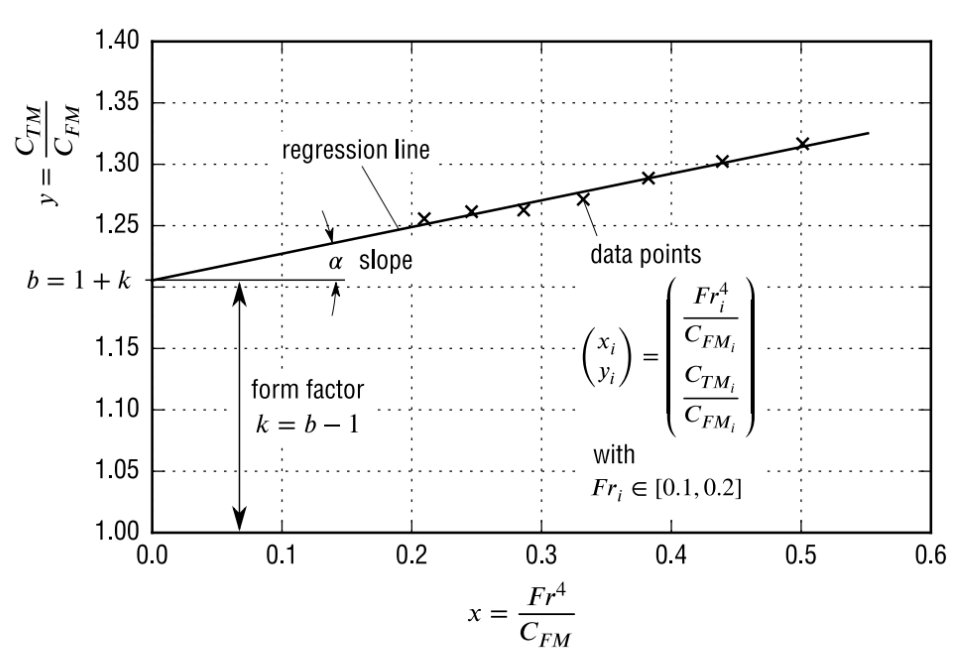
\includegraphics[width=0.65\textwidth]{images/prohaska_diagram}
    \caption{Diagrama del método de Prohaska. Adaptado de \citet{birk2019}.}
    \label{fig:prohaska_esquema}
\end{figure}

El método presenta, sin embargo, limitaciones bien documentadas. La sensibilidad del método a pequeñas incertidumbres de medición es elevada precisamente donde la señal de fuerza es más baja. Las fuentes de desviación pueden agruparse en tres categorías.

La primera corresponde a efectos geométricos no lineales. La presencia de proas bulbo (protuberancias redondeadas ubicadas en la parte sumergida de la proa, concebidas para generar un sistema de olas que interfiere con el del casco y reduce la resistencia por generación de olas) próximas a la superficie libre genera no linealidades en la curva a bajas velocidades que dificultan la extrapolación \citep{korkmaz_cfd_2021}. En \citet{korkmaz_cfd_2021} se analizaron dos modelos con geometrías casi idénticas (95\% de similitud) que mostraron comportamientos divergentes en la determinación del factor de forma mediante el método de Prohaska. Como se observa en la Figura~\ref{fig:korkmaz_bulb_effect}, el primer modelo (Hull-1) presentó una marcada concavidad en la gráfica de $C_T/C_{F0}$ frente a $Fr^n/C_{F0}$ dentro del rango $0.1 < Fr < 0.2$, mientras que el segundo (Hull-2) mantuvo una tendencia lineal. Esta anomalía en el primer caso se atribuyó a un diseño de bulbo tipo ``goose-neck'' con mayor concentración de volumen cerca de la superficie libre, lo cual genera sistemas de ondas cortos que no interactúan favorablemente con el tren de ondas de la proa a bajas velocidades. Este fenómeno se intensificó al ensayar el modelo en condición de lastre, donde la proximidad del bulbo a la superficie libre indujo una protuberancia significativa en la curva, dificultando la extrapolación precisa de la resistencia viscosa.

La segunda fuente de desviación proviene de fenómenos viscosos asociados a la separación del flujo. Cualquier aparición de separación o desprendimiento de vórtices a baja velocidad contradice el supuesto fundamental del método, que presupone un flujo adherido en la condición de referencia. Los cascos con formas llenas pueden presentar pequeñas zonas de separación en la popa o bajo el espejo, especialmente cuando existen apéndices. Las observaciones originales de Prohaska sobre curvas convexas en buques de doble hélice responden a este tipo de efectos: los soportes, ejes o popas voluminosas generaban una resistencia adicional por presión (resistencia por vórtices) incluso a bajos $Fr$, resultando en valores de $C_T$ superiores a los esperados por fricción pura. De manera similar, la separación de flujo en popas espejo sumergidas genera no linealidades \citep{keh-sik-min, korkmaz_cfd_2021}. Una popa espejo parcialmente sumergida puede inducir separación en la estela a escala modelo, fenómeno que no necesariamente se reproduce a escala buque debido a diferencias en el número de Reynolds. Estos efectos, esencialmente viscosos, se traducen en un ``abultamiento'' en la curva de Prohaska por la aparición de un componente adicional de resistencia de forma. Prohaska advirtió que su método no debía aplicarse de forma automática cuando existe separación de flujo, señalando la dificultad de detectar estos fenómenos (por ejemplo, el desprendimiento en popas espejo o zonas de spray separadas en bulbos apenas aflorantes). Estudios más recientes de CFD \citep{korkmaz-verif-and-valid-cfd-efd} confirman que separaciones leves pueden provocar una disminución aparente del factor de forma al aumentar el número de Reynolds, dado que el flujo tiende a re-adherirse progresivamente a mayor velocidad.

La tercera fuente de desviación es de naturaleza analítica y se desdobla, a su vez, en dos aportes. Por un lado, la línea de referencia interviene en el denominador del diagrama: con la ITTC-57, cuya pendiente a bajos $Re$ ya se discutió en la Sección~\ref{sec:ITTC57}, los puntos adquieren una curvatura convexa que no responde al comportamiento del casco \citep{ITTC_Combined_2021}. Por otro, la propia formulación de Prohaska supone que la resistencia por olas varía como ${\sim}Fr^4$; si la ley real difiere de esa potencia --por ejemplo, por la presencia de un sistema secundario de ondas-- los puntos experimentales se apartan de la linealidad esperada, con independencia de la línea de fricción empleada.

% ---------------------------------------------------------------------
% [CORREGIDO] Se explicita cuáles de las tres fuentes intervienen en los
% cascos de esta tesis y dónde se aborda cada una.
% ---------------------------------------------------------------------
Las tres fuentes intervienen simultáneamente en los pesqueros de baja esbeltez
analizados en esta tesis, y su tratamiento organiza buena parte del
Capítulo~\ref{cap:resistencia_factor_de_forma}: la primera a través de la proa
bulbo, cuyo efecto sobre el diagrama de Prohaska se aísla comparando el casco
original con una variante sin bulbo (Sección~\ref{sec:proa_bulbo}); la segunda a
través de la popa espejo, que en la condición de plena carga queda
sustancialmente sumergida y genera separación (Sección~\ref{sec:popa_sumergida});
y la tercera a través de la sensibilidad del valor de $(1+k)$ al rango de Froude
retenido en la regresión. Una primera cuantificación conjunta de estos efectos
para esta clase de cascos se presentó en \citet{oyuela2024jmse}.

\begin{figure}[htbp]
    \centering
    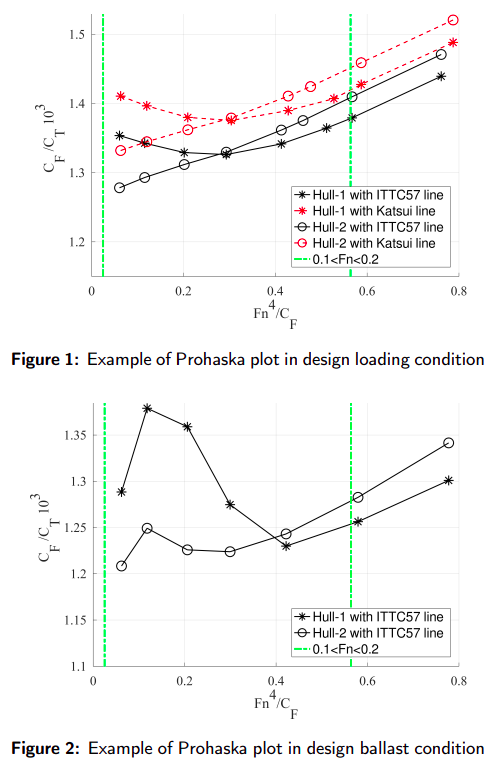
\includegraphics[width=0.6\textwidth]{images/prohaska-korkmaz.png}
    \caption{Diagramas de Prohaska de los modelos Hull-1 y Hull-2. Adaptado de
    \citet{korkmaz_cfd_2021}.}
    \label{fig:korkmaz_bulb_effect}
\end{figure}

\section{Determinación del factor de forma asistida por CFD}
\label{sec:cfd_ff_antec}

El recurso al CFD para determinar el factor de forma plantea dos cuestiones
independientes, que se corresponden con los dos miembros del cociente
$(1+k) = C_V/C_{F0}$ de la Ecuación~\eqref{eq:k_dos_cocientes}. La primera es
cómo obtener el numerador, es decir por qué camino se llega a la resistencia
viscosa $C_V$. Hay dos posibles: reproducir numéricamente el ensayo de remolque
--con superficie libre, sobre el mismo rango de bajos $Fr$ que la campaña
experimental-- y aplicar sobre los resultados el método de Prohaska igual que
sobre datos medidos, o bien eliminar la superficie libre del problema y calcular
$C_V$ de forma directa, que es el enfoque de doble cuerpo. La segunda cuestión es
cuál adoptar como denominador: la línea de fricción de referencia $C_{F0}$ deja
de ser un dato heredado de la práctica experimental y pasa a poder calcularse con
el mismo código y el mismo modelo de turbulencia que se emplean para el casco.
Ambas cuestiones se tratan a continuación por separado.

\subsection{Líneas de fricción numéricas}
\label{sec:nfl_antec}

Cualquiera sea la vía por la que se obtenga $C_V$, el cociente $C_V/C_{F0}$ que
define el factor de forma queda referido a una línea de fricción de origen
distinto al del numerador: $C_V$ sale de una simulación y $C_{F0}$, si se adopta
la ITTC-57, de una correlación experimental que además embebe un factor de forma.
Para evitar esa inconsistencia se han derivado diversas \textbf{líneas de fricción numéricas}
(``Numerical Friction Lines'', NFL) mediante simulaciones CFD de placa plana a
distintos Reynolds \citep{wang2015numericalFL, Korkmaz2019NumericalFL}. A
diferencia de la ITTC-57, no incorporan ningún margen de correlación: son
fricción de placa plana pura, calculada con el mismo código y el mismo modelo de
turbulencia que luego se emplea para el casco. Las
diferencias entre formulaciones se concentran en el rango de números de Reynolds
propio de los modelos de laboratorio y se atenúan marcadamente hacia la escala
buque. La Figura~\ref{fig:lineas_friccion} compara el coeficiente de fricción
$C_F$ de varias de estas líneas (la NFL $k$--$\omega$ SST de
\citet{wang2015numericalFL}, la NFL $k$--$\omega$ SST de \citet{eca2008friction}
y la NFL con el modelo EASM de \citet{Korkmaz2019NumericalFL}) tomando como
referencia la línea ITTC-57. Se observa que todas las líneas numéricas predicen
valores de $C_F$ inferiores a los de la ITTC-57 en el rango de bajos $Re$. Las
distintas NFL $k$--$\omega$ SST coinciden entre sí dentro de un margen del orden
del $2\%$, mientras que la formulación EASM se aparta ligeramente, evidenciando
la influencia del modelo de turbulencia empleado en la derivación
\citep{korkmaz2023thesis}. Hacia el régimen de escala buque las diferencias
entre todas las formulaciones se reducen de manera considerable.

\begin{figure}[htpb]
    \centering
    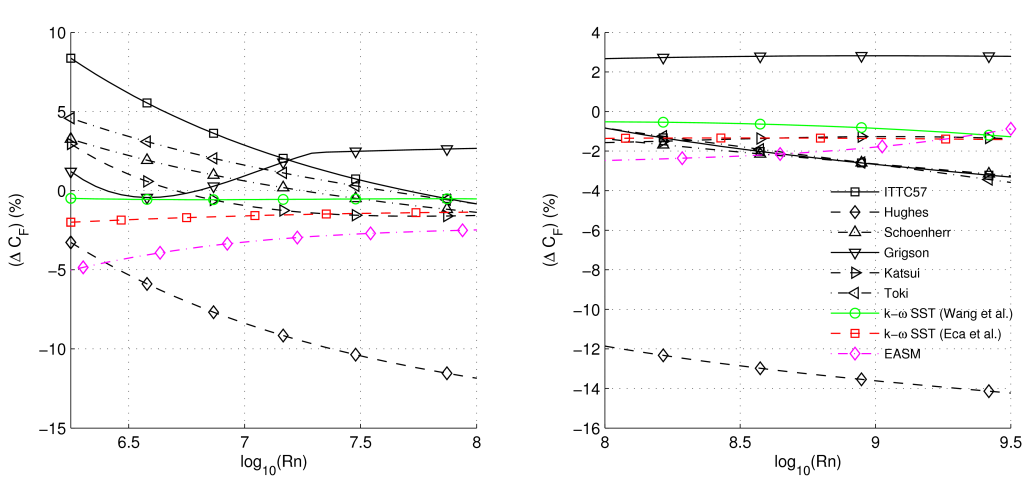
\includegraphics[width=0.7\textwidth]{images/comparacion_lineas_friccion.png}
    \caption{Líneas de fricción numéricas frente a la línea ITTC-57. Adaptado de
    \citet{korkmaz2023thesis}.}
    \label{fig:lineas_friccion}
\end{figure}

En esta tesis las NFL no reemplazan a la línea de referencia adoptada, sino que
se emplean como herramienta de diagnóstico: comparar el factor de forma obtenido
con una y con otra permite separar lo que en su comportamiento con la escala es
atribuible a la línea de referencia de lo que responde a la física del flujo
(Sección~\ref{sec:k_vs_Re}).

\subsection{El enfoque de doble cuerpo}
\label{sec:doble_cuerpo_antec}

% ---------------------------------------------------------------------
% [CORREGIDO] La analogía se establece con el MÉTODO DE BAJAS VELOCIDADES
% (que sí supone C_W despreciable), no con la descomposición de Hughes.
% ---------------------------------------------------------------------
El enfoque de doble cuerpo persigue el mismo objetivo que el método de Prohaska
--acceder a la resistencia viscosa sin la contaminación de la componente por
olas-- pero lo alcanza por una vía que no es equivalente en rigor. Prohaska lo
hace de forma indirecta: supone para $C_W$ una ley de potencia en $Fr$ y la
sustrae por extrapolación, de modo que el valor obtenido depende del rango de
velocidades retenido y de que la ley supuesta describa bien el tren de olas real.
La configuración de doble cuerpo, en cambio, elimina la generación de olas por
construcción, al reemplazar la superficie libre por un plano de simetría: allí
$C_W = 0$ de manera exacta, y no por aproximación ni por sustracción. Esto libera
además al método de toda restricción sobre el número de Froude, ya que puede
computarse cualquier velocidad --y, de hecho, cualquier número de Reynolds,
incluido el del buque-- con la única condición de que el flujo sea turbulento.

Formalmente, al anularse la generación de olas, la resistencia
total obtenida en esta configuración corresponde únicamente a la componente
viscosa, y el factor de forma se obtiene como \citep{ITTC_Combined_2021}:
%
\begin{equation}
    (1+k) = \frac{C_V}{C_{F0}} = \frac{C_F + C_{PV}}{C_{F0}},
\end{equation}
%
donde $C_V = C_F + C_{PV}$ es el coeficiente de resistencia viscosa obtenido de la simulación de doble cuerpo y $C_{F0}$ el coeficiente de la línea de referencia. La ventaja decisiva sobre el método de Prohaska es que el doble cuerpo elimina la contaminación por olas en la determinación de $C_V$ (la mayor fuente de incertidumbre de Prohaska a bajas velocidades) en lugar de intentar sustraerla por extrapolación. La configuración permite además concentrar la resolución de la malla en la capa límite y la estela viscosa de popa, optimizando el costo computacional frente a las simulaciones con superficie libre. Cabe señalar, sin embargo, que la condición de simetría impuesta en la frontera superior puede distorsionar el campo de presiones en la zona de la proa bulbo cuando esta se encuentra próxima a la superficie libre, por lo que su aplicación requiere verificar que la geometría simulada no se vea afectada por esta limitación. En efecto, en \citet{quintuna2023} se observó que, cuando existe un pequeño espacio entre el tope del bulbo y la superficie libre en reposo, la tapa rígida induce una separación de flujo en torno al bulbo que no se produce en las simulaciones con superficie libre, y que este efecto se atenúa al aumentar la inmersión de la proa mediante el asiento, en línea con lo señalado en \citet{korkmaz_cfd_2021}.

\subsection{Resultados disponibles: de los cascos de referencia a los pesqueros de baja esbeltez}
\label{sec:estado_arte_ff}

El Comité Especialista de la 29a ITTC sobre Métodos Combinados CFD/EFD coordinó un
estudio colaborativo en el que nueve organizaciones y ocho códigos calcularon el
factor de forma para los cascos \textit{KCS} y KVLCC2 \citep{ITTC_Combined_2021,
KORKMAZ2022112590}. Los resultados mostraron que la dispersión entre
organizaciones es significativamente menor que la del método de Prohaska, que el
valor medio de las predicciones CFD concuerda con el experimental dentro de la
incertidumbre, y que las predicciones de potencia a escala buque mejoran de manera
generalizada al utilizar factores de forma basados en CFD. Con base en estos
resultados, la ITTC recomienda el uso del CFD como complemento al método
experimental.

Esa evidencia proviene, sin embargo, de cascos de esbeltez moderada. Para cascos
pesqueros con $L/B < 4$ el punto de partida es \citet{oyuela2024jmse}, donde se
determinó el factor de forma de un pesquero por el método de doble cuerpo y se lo
contrastó con el obtenido experimentalmente sobre el mismo casco en el LabHiNO
(Laboratorio de Hidrodinámica Naval y Oceánica, UBA), verificando que el CFD
reproduce el valor medido. Trabajos posteriores del mismo grupo ampliaron el
análisis a la influencia del modelo de turbulencia \citep{oyuela2025mecanica} y a
la comparación con el \textit{KCS} \citep{oyuela2026oceaneng}, que permite situar
el comportamiento de estos cascos frente al de una geometría de referencia.

La ventaja del doble cuerpo frente a Prohaska en esta clase de buques no reside en
una mayor exactitud intrínseca, sino en que suprime la principal fuente de
ambigüedad del método experimental: al no requerir extrapolación desde el rango de
bajos $Fr$, el valor de $(1+k)$ deja de depender de qué puntos se retienen en la
regresión, dependencia que resulta particularmente marcada cuando el espejo de
popa está sustancialmente sumergido. La contrapartida es que la configuración de
doble cuerpo introduce su propia idealización en esa misma zona --la tapa rígida
impone un plano de simetría allí donde el espejo interrumpe la superficie libre--,
de modo que ambos métodos deben leerse como complementarios y no como sustitutos.
Esta comparación se retoma, con los resultados propios, en el
Capítulo~\ref{cap:resistencia_factor_de_forma}.

\section{Dependencia del factor de forma con el número de Reynolds}
\label{sec:k_vs_Re}

Presentado el método completo y sus variantes de determinación, corresponde
examinar el único supuesto que no puede contrastarse dentro del propio ensayo:
que el factor de forma determinado sobre el modelo es el mismo que gobierna el
flujo alrededor del buque, $k_M = k_S$. La evidencia acumulada en las últimas
décadas indica que el factor de forma \emph{aparente} --el que resulta de
aplicar los procedimientos descritos con la línea ITTC-57-- no es constante,
sino que crece de manera sistemática con el número de Reynolds, de modo que
$k_M < k_S$.

Conviene precisar dónde se introduce el error que esto acarrea. El valor
determinado sobre el modelo es el correcto para despejar $C_W$ del ensayo, porque
$k_M$ es justamente el factor de forma que gobierna el flujo a esa escala; el
término de olas se traslada entonces al buque sin error. La discrepancia aparece
recién al recomponer el coeficiente del buque, donde la
Ecuación~\eqref{eq:extrapolacion_CTS} emplea $(1+k_M)$ allí donde correspondería
$(1+k_S)$. La diferencia entre la predicción correcta y la estándar vale
$(k_S - k_M)\,C_{F0}(Re_S)$, positiva siempre que $k_S > k_M$: el término viscoso
de escala buque queda subestimado, y con él la resistencia total del buque.

Dos mecanismos independientes explican por qué cabe esperar esta dependencia.
El primero es físico: el flujo en el modelo está necesariamente a menor número
de Reynolds que en el buque, lo que implica que la capa límite es
proporcionalmente más gruesa, el gradiente de presión adverso en la popa está
más amortiguado y la posible zona de separación es más extensa en el modelo que
en el buque. El segundo es metodológico y remite a las propiedades de la línea de
referencia descritas en la Sección~\ref{sec:ITTC57}, que introducen una
distorsión sistemática en el valor de $k$ calculado con ella. Ambos efectos
actúan en el mismo sentido, $k_M < k_S$.

La cuantificación sistemática de este efecto fue abordada por primera vez en
\citet{gomezgarcia}, donde se reanalizaron quince modelos agrupados en cuatro
familias de modelos geométricamente semejantes a distinta escala. Para cada
familia, el factor de forma determinado por Prohaska con la ITTC-57 disminuye al
aumentar la razón de escala $\lambda$ --equivalentemente, crece con el tamaño
del modelo--, de modo que la extrapolación de la recta de regresión a
$\lambda = 1$ predice un factor de forma de buque mayor que el de cualquier
modelo. El efecto de escala resultante, $k_S - k_M$, crece linealmente con
$\lambda$ (Figura~\ref{fig:gomez-garcia}). Forzando la recta por su valor
teórico en el origen ($k_S - k_M = 0$ para $\lambda = 1$), en
\citet{gomezgarcia} se propone la forma práctica
%
\begin{equation}
    k_S - k_M = 1.91\,(\lambda - 1)\times 10^{-3},
    \label{eq:gomezgarcia}
\end{equation}
%
positiva para todo modelo ($\lambda > 1$), lo que confirma $k_M < k_S$. Con la
línea de Schoenherr (otra línea de fricción de placa plana disponible como
referencia, alternativa a la ITTC-57) la pendiente resulta significativamente
menor, dado que sus coeficientes de fricción a $Re$ de modelo son más próximos a
los de escala buque que los de la ITTC-57: un primer indicio de que parte del
efecto no es físico sino atribuible a la referencia elegida. En
\citet{ITTC_Combined_2021} se estimó que una extrapolación estándar con factor
de forma constante puede subestimar la resistencia del buque en hasta un 10\%.

\begin{figure}[htpb]
\centering
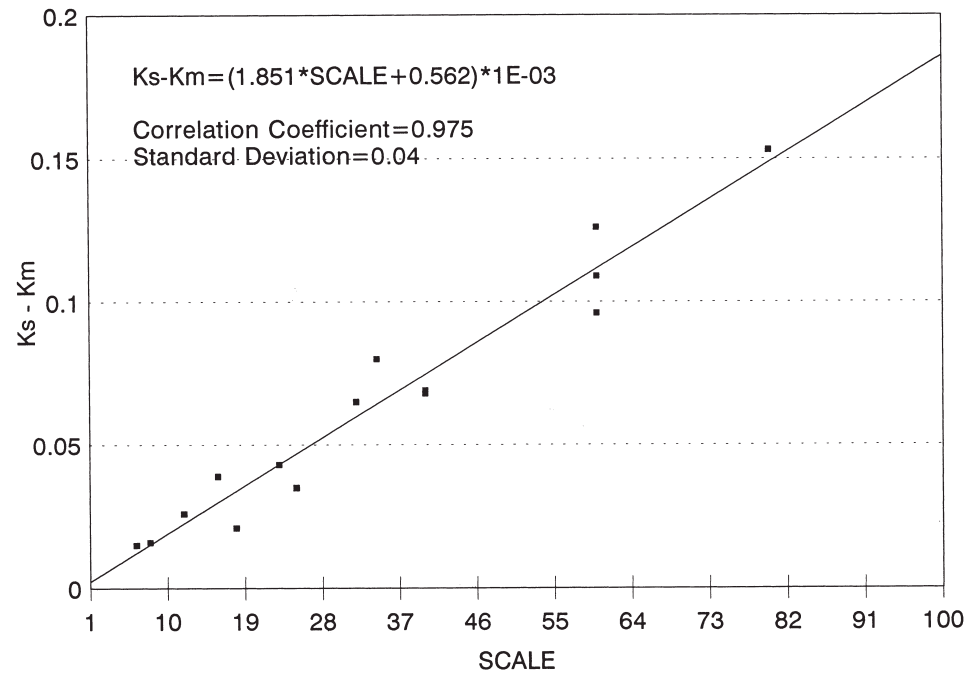
\includegraphics[width=0.6\textwidth]{images/gomez-garcia.png}
\caption{Efecto de escala del factor de forma en función de la razón de escala.
Adaptado de \citet{gomezgarcia}.}
\label{fig:gomez-garcia}
\end{figure}

Un programa experimental de alcance comparable, extendido entre 1992 y 2006, se
presenta en \citet{keh-sik-min}: doce buques de distinto tipo ensayados sobre un
total de 32 modelos, construidos en varias escalas para un mismo casco de modo
de barrer el número de Reynolds manteniendo el de Froude. La Figura~\ref{fig:keh-sik} reproduce los resultados de los ensayos de baja
velocidad para los cuatro modelos geosim de un portacontenedores de 8600~TEU,
graficados como $C_{TM}/C_{FM}$ frente a $Fr$. En ese plano, el valor al que
tiende cada curva cuando $Fr \to 0$ es el factor de forma, según la definición
adoptada por la ITTC en 1978 y empleada por los autores. Dos rasgos son
relevantes. El primero es que ese valor asintótico crece de manera sistemática
con la eslora del modelo --y por lo tanto con $Re$--: aplicando su procedimiento
estándar, los autores obtienen $1.008$ y $1.012$ en los modelos de 2 y 4~m frente
a $1.102$ y $1.124$ en los de 7.6 y 10~m para un mismo buque. El segundo es que
las curvas de los dos modelos pequeños son cualitativamente distintas de las de
los grandes: presentan una caída pronunciada y un quiebre por debajo de
$Fr \approx 0.06$ que las curvas de los modelos mayores no exhiben. Los propios autores atribuyen ese comportamiento a
que, con números de Reynolds del orden de $10^5$, el flujo alrededor de los
modelos pequeños es mayormente laminar o transicional.

\begin{figure}[htbp]
\centering
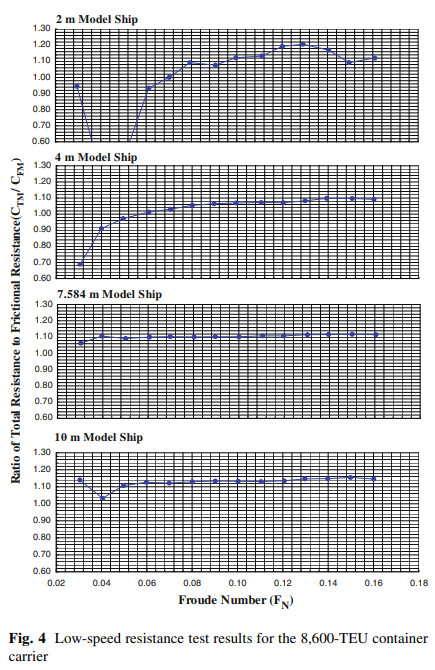
\includegraphics[width=0.6\textwidth]{images/keh-sik-min.png}
\caption{Ensayos de baja velocidad de los cuatro modelos geosim del
portacontenedores de 8600~TEU. Adaptado de \citet{keh-sik-min}.}
\label{fig:keh-sik}
\end{figure}

Sobre esta base, en \citet{keh-sik-min} se propone un \textbf{factor de forma
terminal}, definido como el valor al que tiende $(1+k)$ cuando el flujo alcanza
el régimen plenamente turbulento --que los autores sitúan en $Re \sim 10^9$, y
que en la práctica corresponde al buque a velocidad de diseño--, y un
\textbf{factor de corrección} que permite llevar el valor medido en la escala de
ensayo hasta ese valor terminal. La curva de corrección, ajustada por una
función tangente hiperbólica del logaritmo de $Re$, se muestra en la
Figura~\ref{fig:keh-sik-2}.

Conviene señalar una limitación de esta evidencia, que condiciona la
interpretación tanto de la Figura~\ref{fig:keh-sik} como de la propia curva de
corrección: en esa campaña no se emplearon estimuladores de turbulencia en
ninguno de los modelos. Parte del crecimiento observado de $(1+k)$ con el tamaño
del modelo no responde entonces a una dependencia física del factor de forma con
$Re$, sino a que los modelos pequeños no alcanzan el régimen turbulento sobre el
que la hipótesis de Hughes está formulada. Los propios autores son consistentes
con esta lectura: sostienen que, una vez plenamente turbulento el flujo, el
factor de forma se estabiliza en su valor terminal. Lo que la evidencia
establece con solidez, por lo tanto, no es que $k$ varíe intrínsecamente con el
número de Reynolds, sino algo suficiente para el problema que aquí interesa: que
el valor medido a escala de modelo no es, sin corrección, el valor que gobierna
el flujo alrededor del buque.

\begin{figure}[h]
\centering
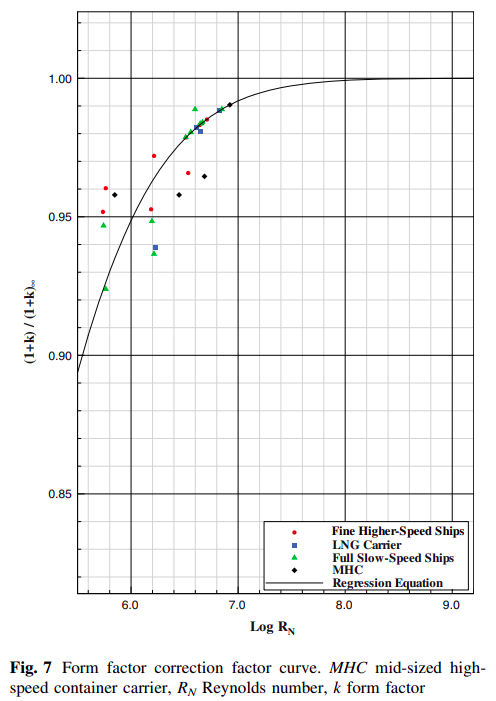
\includegraphics[width=0.6\textwidth]{images/keh-sik-min-2.png}
\caption{Curva del factor de corrección del factor de forma. Adaptado de
\citet{keh-sik-min}.}
\label{fig:keh-sik-2}
\end{figure}

La pregunta clave es en qué medida esta dependencia con $Re$ es un artefacto de la línea de referencia y en qué medida refleja física real. La evidencia acumulada permite separar tres contribuciones distintas. A ellas se agrega, por último, una configuración geométrica particular en la que la segunda de esas contribuciones se vuelve dominante y exige un tratamiento propio.

\subsection{La contribución de la línea de referencia}

El estudio colaborativo ITTC \citep{korkmaz_cfd_2021} aportó evidencia concluyente: la dependencia de $k$ con
$Re$ desaparece casi por completo al reemplazar la ITTC-57 por líneas de
fricción numéricas derivadas con el mismo código, al menos para cascos de
esbeltez moderada como el \textit{KCS} y el KVLCC2. Esto indica que la mayor
parte de la dependencia observada es un artefacto de la pendiente incorrecta de
la ITTC-57 a bajos números de Reynolds, y no un efecto físico inherente. En la
misma dirección, en \citet{quintuna2023} se determinaron factores de forma por
CFD de doble cuerpo para un buque multipropósito y un portacontenedores, y se
cuantificó que la diferencia del factor de forma entre escala modelo y escala
buque se reduce en promedio del $10.4\%$, al emplear la línea ITTC-57, al
$6.4\%$ al utilizar una NFL derivada con el modelo $k$--$\omega$ SST.

Estas cifras admiten, sin embargo, una segunda lectura: la reducción es
sustancial pero no completa, y la fracción remanente no puede atribuirse a la
referencia. En efecto, la mejora no es universal. En configuraciones con
apéndices, o en cascos donde la resistencia por presión viscosa $C_{PV}$
constituye una fracción significativa de la resistencia viscosa total, el factor
de forma continúa mostrando variaciones apreciables con el número de Reynolds
incluso al emplear NFL, lo que indica que la hipótesis de proporcionalidad entre
resistencia viscosa y fricción de placa plana resulta insuficiente en flujos
tridimensionales complejos \citep{wang2015numericalFL}. Este es precisamente el
caso de los pesqueros de baja esbeltez analizados en esta tesis, como se
documenta en el Capítulo~\ref{cap:resistencia_factor_de_forma}.

\subsection{La contribución física asociada a la forma del casco}

% ---------------------------------------------------------------------
% [REESCRITO] Sin referencia al método de Froude: todo el argumento se
% expresa dentro de la descomposición de Hughes.
% ---------------------------------------------------------------------
La contribución analizada en el apartado anterior afecta al primer término de la
Ecuación~\eqref{eq:k_dos_cocientes}: una línea de referencia con pendiente
incorrecta hace que $C_F/C_{F0}$ varíe con $Re$ aun cuando la física del casco
sea la esperada. El segundo término, en cambio, no se corrige cambiando la
referencia. Sostener $k_M = k_S$ exige también que la resistencia por presión
viscosa $C_{PV}$ mantenga una proporción invariante al aumentar el número de
Reynolds, y es ahí donde interviene la forma del casco.

En \citet{DOGRUL2020107428} se calcularon por CFD de doble cuerpo los factores
de forma del \textit{KCS} y del KVLCC2 en tres escalas de modelo y en escala
real, empleando como referencia tanto la línea ITTC-57 como la ATTC-1947. El
resultado directo es que $(1+k)$ crece de manera monótona con $Re$ en ambos
cascos: con la ITTC-57, aproximadamente de $1.10$ a $1.16$ en el \textit{KCS} y
de $1.20$ a $1.27$ en el KVLCC2 entre el modelo más pequeño y la escala buque. La
comparación entre ambas líneas de referencia reproduce, de paso, el
comportamiento descrito en el apartado anterior: las diferencias entre los
valores obtenidos con una y otra son apreciables en el rango de Reynolds de
modelo y se anulan en escala buque, donde las dos líneas de fricción convergen.

Las simulaciones con superficie libre del mismo trabajo permiten ubicar ese
crecimiento en el segundo término de la Ecuación~\eqref{eq:k_dos_cocientes}. Por
un lado, el coeficiente de fricción calculado sobre el casco se aproxima
estrechamente a la línea ITTC-57 en todas las escalas, de modo que el cociente
$C_F/C_{F0}$ no aporta una variación apreciable. Por otro, la resistencia por
presión viscosa disminuye de manera sistemática con $Re$ en ambos cascos, en
correspondencia con una recuperación de presión más completa en la popa a medida
que la capa límite se adelgaza. El efecto neto es que $C_{PV}$ decrece, pero más
lentamente que la fricción de referencia, y el cociente $C_{PV}/C_{F0}$ --es
decir, el factor de forma-- crece con la escala.

La forma del casco no interviene en el signo de este efecto, que es el mismo en
ambos buques, sino en el peso que el segundo término tiene sobre el total. La
presión viscosa representa alrededor del $7\%$ de la resistencia total del
\textit{KCS} en todas las escalas, frente a un $16$--$17\%$ en el KVLCC2, de
formas mucho más llenas; los factores de forma correspondientes son también
mayores en este último. Cuanto mayor es esa fracción, mayor es la porción de
$(1+k)$ que queda gobernada por un término que no escala como la fricción, y
menos margen hay para tratar el factor de forma como una constante puramente
geométrica. Los cascos pesqueros de muy baja esbeltez analizados en esta tesis se
ubican en el extremo de esa tendencia, y es ésta la razón por la cual corregir la
línea de referencia no basta para estabilizar su factor de forma, como se
documenta en el Capítulo~\ref{cap:resistencia_factor_de_forma}.

\subsection{El comportamiento a muy bajos números de Froude}

En \citet{TERZIEV2021147} se abordó esta cuestión numéricamente, calculando por
doble cuerpo el factor de forma de una serie geosim del \textit{KCS} sobre cuatro
factores de escala ($\lambda = 75$, $52.667$, $31.599$ y $1$), catorce números de
Froude entre $0.02$ y $0.28$ y tres modelos de turbulencia ($k$-$\omega$,
$k$-$\varepsilon$ y $k$-$\omega$ SST). El estudio se complementó con simulaciones
de escalado viscoso, en las que el número de Reynolds se altera modificando la
viscosidad del fluido a Froude fijo, lo que permite separar ambos efectos de un
modo inaccesible experimentalmente.

El trabajo reporta, en efecto, una dependencia con el número de Froude, pero
acotada en su alcance. La variación se concentra en el rango $Fr = 0.02$--$0.06$,
donde las diferencias entre velocidades adyacentes alcanzan el $10$--$20\%$, con
un máximo del $20.9\%$; por encima de ese rango caen por debajo del $1\%$, y el
escalado viscoso no detecta efecto alguno entre $Fr = 0.26$ y $0.28$.

Los propios autores matizan además ese hallazgo. La incertidumbre numérica se
mantiene por debajo del $2\%$ en la mayoría de los casos, pero los valores
atípicos por encima del $5\%$ provienen exclusivamente de ese mismo extremo
inferior, lo que indica que el método RANS se ve más exigido allí que a
velocidades intermedias o altas. Y la dispersión entre modelos de turbulencia
resulta mayor que la atribuible al Froude: a $\lambda = 75$ y $Fr = 0.02$ el
factor de forma pasa de $1.029$ con el modelo SST a $1.185$ con el
$k$-$\varepsilon$, una diferencia que excede las bandas de incertidumbre de ambos.
Señalan que ello dificulta sostener argumentos concretos en esa región, y cierran
indicando que la naturaleza del efecto de escala sobre el factor de forma, tanto
en Froude como en Reynolds, requiere investigación adicional. Para lo que aquí
interesa, la consecuencia es que el rango en el que la variación se manifiesta
queda por debajo de la ventana $Fr \in [0.1;\, 0.2]$ sobre la que opera el método
de Prohaska, dentro de la cual las diferencias reportadas son de unos pocos por
ciento.
\subsection{Una configuración particular: la popa espejo sumergida}

Cuando la popa del casco tiene el espejo sumergido, el flujo se separa en la arista y se forma detrás una zona de recirculación persistente. La inmersión del espejo se acentúa al aumentar el calado y al reducir la velocidad, de modo que el régimen recirculante es más probable en condición de plena carga y, dentro de ella, justamente en el rango de bajos $Fr$ sobre el que operan los métodos de determinación de $(1+k)$. En esa configuración, el flujo de escala modelo y el flujo de escala buque difieren cualitativamente, no solo cuantitativamente, porque la velocidad crítica a la que el espejo ``ventila'' y pasa a flujo libre es diferente en las dos escalas \citep{ITTC_Combined_2021}. Para este caso, en \citet{korkmaz_wetted_transom} se propone un \textbf{método de dos factores de forma} ($2k$) que distingue la contribución del cuerpo sin separación de la contribución adicional de la popa espejo, calculando ambas por CFD en escala modelo y buque respectivamente. El método incluye un criterio de aplicabilidad basado en el área sumergida del espejo relativa a la sección maestra. Los cascos pesqueros analizados en esta tesis superan ese umbral en su condición de plena carga, de modo que la corrección corresponde ser aplicada; cuánto explica del efecto de escala medido en ellos es una cuestión distinta, que se cuantifica en la Sección~\ref{sec:popa_sumergida}.

Recientemente en \citet{starke2025} se propuso una variante en la que el factor de forma se calcula sobre una versión del casco con la popa geométricamente cerrada, dejando la resistencia de la popa espejo fuera del escalado viscoso (verificada sobre diez cascos, reduce la subestimación de la resistencia a escala buque a un $0$--$3\%$). Su comparación sistemática con el método de dos factores de forma para los cascos aquí estudiados queda como línea de trabajo futuro.
 
 
\section{Hidrodinámica de hélices en aguas abiertas}
\label{sec:helices_antec}
 
\subsection{Coeficientes adimensionales y ensayo en aguas abiertas}
\label{sec:pow_antec}
 
El comportamiento hidrodinámico de una hélice se caracteriza a través de su \textbf{diagrama de aguas abiertas} (``Propeller Open Water diagram'', POW), obtenido en ensayos donde la hélice opera en flujo uniforme sin influencia del casco. Las variables de interés son el coeficiente de empuje $K_T$, el coeficiente de par $K_Q$ y la eficiencia en aguas abiertas $\eta_0$:
%
\begin{equation}
    K_T = \frac{T}{\rho n^2 D^4}, \qquad
    K_Q = \frac{Q}{\rho n^2 D^5}, \qquad
    \eta_0 = \frac{K_T}{K_Q}\,\frac{J}{2\pi},
\end{equation}
%
donde $T$ es el empuje, $Q$ el par, $\rho$ la densidad del fluido, $n$ la velocidad de giro en rev/s, $D$ el diámetro y $J = V_a/(nD)$ el coeficiente de avance, con $V_a$ la velocidad de avance del flujo incidente. Se denota $R = D/2$ el radio de la pala y $r$ la coordenada radial medida desde el eje, de modo que $r/R$ es la posición radial adimensional que identifica cada sección de la pala.

La caracterización del régimen de flujo sobre la pala admite dos números de Reynolds de uso corriente, que conviene distinguir explícitamente porque no son intercambiables. El primero es el \textbf{número de Reynolds rotacional},
%
\begin{equation} \label{eq:Re_rotacional}
    Re_n = \frac{n D^2}{\nu},
\end{equation}
%
construido únicamente con parámetros globales de operación y empleado para identificar el punto de funcionamiento de una campaña completa. El segundo es el \textbf{número de Reynolds seccional}, definido sobre una sección concreta de la pala. Para la sección ubicada en la posición radial $r/R$ se denota $c_{r/R}$ la longitud de su cuerda, es decir la distancia entre el borde de ataque y el borde de salida del perfil que resulta de cortar la pala a ese radio, que es la dimensión característica sobre la que se desarrolla la capa límite en esa sección:
%
\begin{equation} \label{eq:Re_helice}
    Re_c = \frac{c_{r/R}\, V_{r/R}}{\nu}, \qquad V_{r/R} = \sqrt{V_a^2 + \left(\pi n D\, \tfrac{r}{R}\right)^2},
\end{equation}
%
donde $V_{r/R}$ es la velocidad resultante del flujo incidente sobre esa sección, compuesta por la velocidad de avance y la velocidad tangencial de rotación. Este último es el que gobierna el estado de la capa límite sobre la pala y, por lo tanto, el que aparece en los criterios de representatividad de los ensayos y en el procedimiento de extrapolación. Dado que la sección de referencia no es la misma en todos los procedimientos --la ITTC evalúa la representatividad del ensayo de aguas abiertas a $r/R = 0.7$ y construye la corrección de arrastre del procedimiento ITTC-78 a $r/R = 0.75$--, se indica en cada caso la sección empleada mediante la notación $Re_{c,0.7R}$ y $Re_{c,0.75R}$ \citep{ITTC_Performance_prediction}.
 
\subsection{La serie Wageningen B}
\label{sec:wageningen_antec}
 
La \textbf{serie Wageningen B} es la familia sistemática de hélices de referencia más ampliamente utilizada en la industria naval. Comprende modelos experimentados en el canal MARIN cubriendo de $Z = 2$ a $Z = 7$ palas, relaciones de área expandida $A_E/A_0$ de $0.30$ a $1.05$ (cociente entre el área expandida de las palas y el área del disco de la hélice) y relaciones paso--diámetro $P/D$ de $0.5$ a $1.4$ (con $P$ el paso geométrico y $D$ el diámetro de la hélice). Los resultados originales de \citet{troost1940} fueron corregidos por efectos de escala y ajustados a polinomios de regresión en \citet{oosterveld1975}, cuyas expresiones para $K_T$ y $K_Q$ en función de $J$, $P/D$, $A_E/A_0$ y $Z$ son actualmente la referencia estándar. Dichos polinomios fueron obtenidos a $Re_{c,0.75R} = 2\times10^6$ y son la base para la hélice B4-60 ($P/D = 0.81$, $D = 0.14$~m) analizada numéricamente en el LabHiNO (Laboratorio de Hidrodinámica Naval y Oceánica, UBA) y presentada en el Capítulo~\ref{chap:helices}. La nomenclatura de la serie identifica, en ese orden, la serie B, el número de palas y la relación de área expandida: B4-60 designa entonces una hélice de cuatro palas con $A_E/A_0 = 0.60$.
 
\section{Efectos de escala en hélices y el procedimiento ITTC-78}
\label{sec:escala_helices}
 
\subsection{El procedimiento ITTC-78 para propulsores}
\label{sec:ittc78_propulsor}
 
El \textbf{procedimiento ITTC-78} extrapola los resultados del ensayo POW de modelo a escala buque asumiendo que toda la diferencia entre escalas es de naturaleza friccional \citep{ITTC_Performance_prediction}. Su único insumo es la corrección del coeficiente de arrastre de perfil de la sección representativa, tomada a $r/R = 0.75$:
%
\begin{equation}
    \Delta C_D = C_{D,M} - C_{D,S},
\end{equation}
%
donde $C_{D,M}$ y $C_{D,S}$ son los coeficientes de arrastre del perfil equivalente en escala modelo y buque, estimados mediante correlaciones de placa plana 2D. El objetivo del método, sin embargo, no es $\Delta C_D$ en sí, sino corregir los coeficientes propulsivos: a partir de esa única diferencia de fricción se calculan las correcciones de empuje y de par, $\Delta K_T$ y $\Delta K_Q$, con las que se ajustan los valores de modelo a escala buque,
%
\begin{equation}
    K_{TS} = K_{TM} - \Delta K_T, \qquad K_{QS} = K_{QM} - \Delta K_Q,
    \label{eq:ittc78_correcciones}
\end{equation}
%
de modo que, siendo $\Delta C_D > 0$, resulta $\Delta K_T < 0$ y $\Delta K_Q > 0$: el empuje aumenta y el par disminuye al pasar de modelo a escala buque. Las expresiones completas de $\Delta K_T$ y $\Delta K_Q$ en función de $\Delta C_D$, junto con las correlaciones de placa plana para $C_{D,M}$ y $C_{D,S}$, se detallan en la Sección~\ref{sec:ittc78_helices_metodo}.
 
Este procedimiento tiene dos limitaciones fundamentales que motivan el trabajo original del Capítulo~\ref{chap:helices}. En primer lugar, ignora los cambios en la distribución de presiones sobre las palas al variar $Re$. En segundo lugar, no contempla el comportamiento no monótono de $K_T$ y $K_Q$ en el rango transicional en el que pueden encontrarse a escala de modelo.
 
\subsection{Insuficiencia de corregir solo fricción: el campo de presiones}
\label{sec:presion_escala}

Al aumentar $Re$ desde escala modelo hacia escala buque, no solo cambia el nivel
de fricción: toda la distribución de presiones sobre la pala se modifica a medida
que la capa límite se adelgaza, la zona de separación en el borde de salida se
reduce y el campo de circulación varía.

En \citet{gallotti2026} se realizó una investigación sistemática por CFD de los
efectos de escala en hélices marinas, definiendo la \textbf{fracción de presión}
$f_p = \Delta K_{Tp}/(\Delta K_{Tp}+\Delta K_{Tf})$ --la porción del incremento de
empuje entre escala de modelo y escala buque atribuible a la componente de
presión-- como métrica cuantitativa del fenómeno. Conviene fijar aquí la
convención de signos, porque difiere de la de la
Ecuación~\eqref{eq:ittc78_correcciones}. En lo que sigue, y en todo el análisis de
efectos de escala del Capítulo~\ref{chap:helices}, $\Delta K_T = K_{TS} - K_{TM}$
denota el \emph{incremento} del coeficiente de empuje al pasar de escala de modelo
($K_{TM}$) a escala buque ($K_{TS}$), cantidad positiva, y se descompone como
$\Delta K_T = \Delta K_{Tp} + \Delta K_{Tf}$ en sus contribuciones de presión y de
fricción, definidas en el Capítulo~\ref{chap:Metodologia}; con esa convención,
$f_p = \Delta K_{Tp}/\Delta K_T$. El procedimiento ITTC-78 adopta en cambio el
signo opuesto, ya que su $\Delta K_T$ es la cantidad que se resta del valor de
modelo para producir ese mismo aumento; al comparar ambos marcos se explicita la
conversión.

El estudio abarca tanto una hélice convencional (VP1304, $A_E/A_0=0.779$, sin
modificación de punta) como una de punta rakeada y área expandida reducida
(P1727, $A_E/A_0=0.444$). El \emph{rake} es el desplazamiento axial de las
secciones de la pala a lo largo del eje; una hélice de punta rakeada concentra ese
desplazamiento en la región exterior, de modo que la punta se inclina hacia proa o
hacia popa respecto del plano del disco en lugar de permanecer contenida en él.
Para el P1727 los autores reportan un incremento de empuje entre escala de modelo
y escala buque de hasta un $10\%$ bajo un modelo completamente turbulento; al
descomponer ese incremento, la fracción de presión resulta $f_p\approx0.87$ (entre
$0.83$ y $0.89$ según el coeficiente de avance), de modo que el procedimiento
ITTC-78, que corrige únicamente la fricción, capta apenas la fracción restante
(del orden del $13\%$).

Es importante notar que la fracción de presión del P1727 responde a dos
mecanismos superpuestos. El primero es el área expandida reducida: para un mismo
diámetro y un mismo empuje, menos área significa cuerdas más cortas, y por lo
tanto números de Reynolds seccionales más bajos y una carga hidrodinámica por
unidad de superficie más alta. La capa límite queda entonces gobernada por
gradientes de presión intensos antes que por la fricción, y es esa distribución de
presiones la que más se modifica al pasar a escala buque. El segundo es el rake de
punta, que a escala buque atenúa la separación en esa región y añade una
contribución de presión adicional propia de las geometrías de punta modificada
\citep{Baltazar2021}. Una hélice de área reducida pero \emph{sin} rake apreciable
comparte solo el primer mecanismo, por lo que cabe esperar para ella una fracción
de presión intermedia entre la de una hélice convencional y la del P1727. Este
marco se retoma en el Capítulo~\ref{chap:helices}, donde el P1727 se emplea como
cota superior y el VP1304 como cota inferior convencional --junto con la serie
Wageningen B4-60-- para acotar la fracción de presión de la hélice de menor
$A_E/A_0$ analizada en esta tesis.

La insuficiencia de la corrección por fricción no se limita a las geometrías de
punta modificada. En \citet{peravali2016} se analizó la hélice Kappel, una
geometría no convencional en la que la punta de la pala se curva de forma continua
hacia el lado de succión, integrando una \emph{aleta} en lugar de terminar en una
punta plana: el efecto viscoso de escala sobre la eficiencia predicho por RANS es
de $3.5\%$ para la Kappel frente a $2\%$ para la hélice convencional, mientras que
el ITTC-78 estima menos del $2\%$ en ambos casos.

El caso de las hélices entubadas ofrece la evidencia más nítida de que el problema es de presión y no
de fricción. En \citet{krasilnikov2016cfd} se realizaron simulaciones CFD
sistemáticas de una hélice de paso controlable operando dentro de dos toberas de
distinto diseño, cubriendo cinco escalas, tres relaciones de paso y cinco
coeficientes de avance, y se descompusieron el empuje de la hélice, el empuje de
la tobera y el par en sus componentes de presión y de fricción. En términos
relativos la componente friccional es la que más cambia, reduciéndose
aproximadamente a la mitad entre escala de modelo y escala buque y siguiendo de
cerca una línea de fricción de placa plana; la de presión varía mucho menos, pero
por ser un orden de magnitud mayor en valor absoluto es la que domina el efecto de
escala sobre el empuje de la tobera, al que aporta más del $80\%$. Al contrastar
sus resultados con el procedimiento ITTC-78, los autores muestran que éste, por no
contemplar el efecto del número de Reynolds sobre la sustentación y por lo tanto
sobre la componente de presión, subestima el efecto de escala sobre el par y
predice un aumento del empuje de la hélice allí donde el CFD predice una
disminución: el error no es de magnitud sino de signo, y de ahí la conclusión de
que las hélices entubadas requieren un procedimiento de escalado propio.

Conviene subrayar que el paralelo con el caso de hélice libre es de mecanismo y no
de signo. En la configuración entubada la aceleración del flujo que provoca la
tobera hace operar a la hélice a un coeficiente de avance efectivo mayor, de modo
que el empuje de la pala \emph{disminuye} a escala buque, mientras que la fracción
de presión de \citet{gallotti2026} está definida sobre un incremento. Lo que
ambos casos comparten, y es lo que aquí interesa, es que el efecto de escala
reside mayoritariamente en una componente de presión que el procedimiento estándar
no corrige.
 
\subsection{El régimen transicional y la joroba en $K_T$/$K_Q$}
\label{sec:chichon_antec}
 
Se aborda aquí la segunda de las dos limitaciones del procedimiento ITTC-78 enunciadas en la Sección~\ref{sec:ittc78_propulsor}. Si la anterior se refería a qué se corrige --solo fricción, cuando también cambia la presión--, ésta se refiere a desde dónde se corrige: al punto de partida del ensayo de modelo, que puede no ser representativo del régimen turbulento que el método supone.

Los ensayos POW se realizan típicamente a $Re_{c,0.7R}$ entre $2\times10^5$ y $2\times10^6$, rango en el que la capa límite sobre las palas puede encontrarse en régimen de transición laminar--turbulenta. En estas condiciones, $K_T$ y $K_Q$ exhiben una dependencia no monótona con $Re_{c,0.7R}$: la transición genera primero un incremento pronunciado en la resistencia de perfil antes de que el flujo se vuelva enteramente turbulento y los coeficientes recuperen una tendencia suave. Esta joroba en las curvas, documentada numéricamente en \citet{baltazar2018transition} y presentada en las Figuras \ref{fig:joroba_kt_joao} y \ref{fig:joroba_kq_joao}, no está contemplada en el método ITTC-78, cuya corrección $\Delta C_D$ asume una variación monótona. Cabe señalar, sin embargo, que en \citet{baltazar2018transition} se dispone de un único punto experimental para validar la variación con $Re_{c,0.7R}$, siendo el resto de la curva de naturaleza puramente numérica. Esta base experimental limitada deja abierta la pregunta sobre si la joroba predicha refleja fielmente el comportamiento real o constituye en parte un artefacto del modelo de transición empleado. La limitación de los modelos de turbulencia estándar para capturar este comportamiento en el rango transicional había sido señalada previamente en \citet{rijpkema2015viscous}, donde se mostró que el modelo SST predice líneas de corriente excesivamente circunferenciales en las palas comparadas con ``paint tests'' experimentales, indicando una sobreestimación del área turbulenta y errores sistemáticos en $K_T$ y $K_Q$ en escala modelo.
 
\begin{figure}[htbp]
    \centering
    \begin{subfigure}[b]{0.48\textwidth}
        \centering
        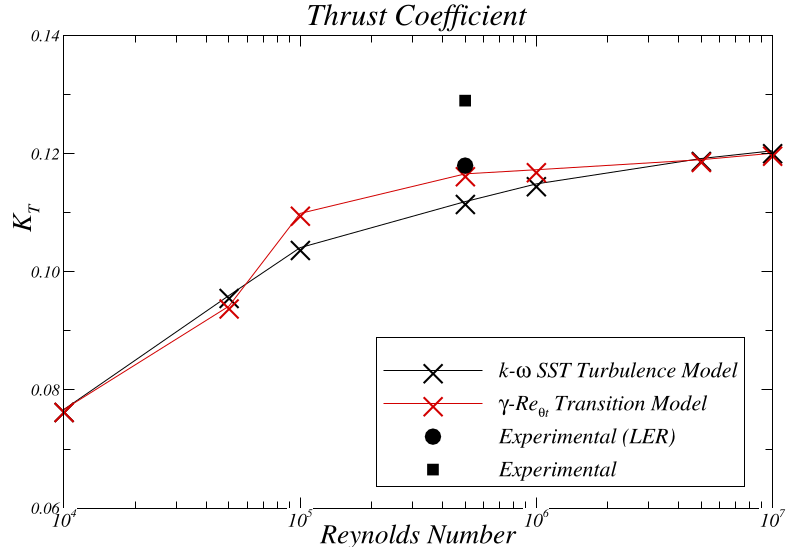
\includegraphics[width=\textwidth]{images/joroba_kt_joao.png}
        \caption{Coeficiente de empuje $K_T$.}
        \label{fig:joroba_kt_joao}
    \end{subfigure}
    \hfill
    \begin{subfigure}[b]{0.48\textwidth}
        \centering
        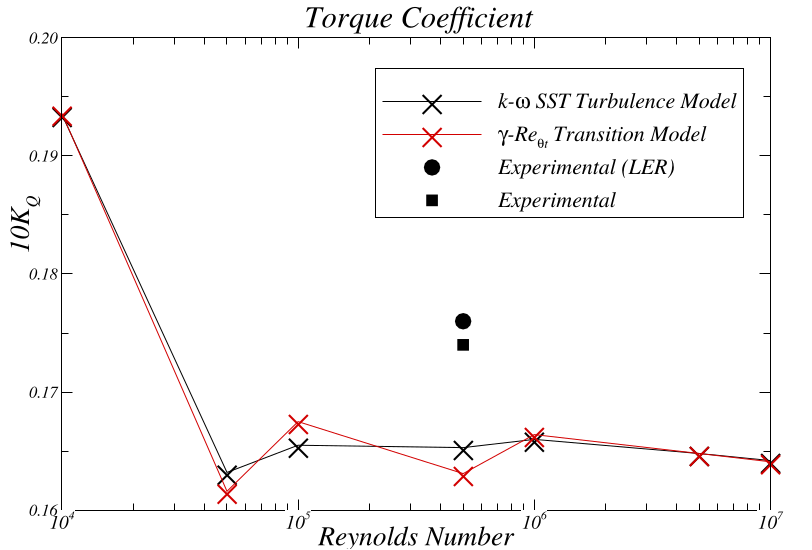
\includegraphics[width=\textwidth]{images/joroba_kq_joao.png}
        \caption{Coeficiente de par $K_Q$.}
        \label{fig:joroba_kq_joao}
    \end{subfigure}
    \caption{Coeficientes de empuje y de par frente al número de Reynolds
    seccional $Re_{c,0.7R}$. Adaptado de \citet{baltazar2018transition}.}
    \label{fig:joroba_joao}
\end{figure}
 
Las referencias fundamentales para la predicción numérica de este fenómeno son \citet{baltazar2018transition} y los trabajos de Gaggero. En \citet{baltazar2018transition} se compararon el modelo SST y el modelo de transición $\gamma$-$\widetilde{Re}_{\theta t}$ (descrito en la Sección~\ref{sec:modelos_transicion}) para dos hélices, obteniendo mejor acuerdo con los diagramas experimentales con el modelo de transición en el rango $Re_{c,0.7R} = 10^5$--$10^6$. Existen otros cierres de transición: en \citet{gaggero2018transition} se empleó en OpenFOAM el modelo $k$-$k_L$-$\omega$, que incorpora una ecuación de transporte adicional para la energía cinética de las fluctuaciones laminares $k_L$. Sus limitaciones fueron señaladas posteriormente en \citet{gaggero2021transition}: el cierre posterga la transición hasta números de Reynolds excesivamente altos --del orden de $2.3\times10^6$ para la hélice VP1304-- y resulta prácticamente insensible a la intensidad turbulenta impuesta en la entrada del dominio.

En \citet{gaggero2021transition} se retomaron esos mismos casos con el modelo $\gamma$-$\widetilde{Re}_{\theta t}$, resuelto tanto en OpenFOAM como en StarCCM+. De ese trabajo interesa aquí sobre todo un resultado: incluir la transición eleva \emph{tanto} $K_T$ \emph{como} $K_Q$ por encima de los valores totalmente turbulentos. Una capa límite parcialmente laminar reduce la fricción, y por sí sola debería producir un leve aumento del empuje junto con una caída más marcada del par; que ambos suban a la vez no se explica por esa vía y obliga a atribuir el efecto a la presión. El mecanismo propuesto es que, bajo capa límite laminar, las líneas de corriente sobre la pala adoptan una orientación predominantemente radial --por el predominio de la fuerza centrífuga-- que produce un efecto equivalente a un aumento de curvatura del perfil y eleva la succión en el dorso, en particular hacia el borde de salida; ese incremento de succión aporta simultáneamente empuje y par, y cancela el efecto favorable de la menor fricción. A diferencia del $k$-$k_L$-$\omega$, este cierre sí exhibe una sensibilidad apreciable a la intensidad turbulenta de entrada, cuestión que se retoma en la Sección~\ref{sec:modelos_transicion}.
 
La implicación directa para la extrapolación ITTC-78 es que, si el ensayo de modelo se realiza en el rango de la joroba, los valores de $K_T$ y $K_Q$ medidos no son representativos del comportamiento turbulento que el método asume y la corrección $\Delta C_D$ puede introducir errores sistemáticos de signo indefinido. Este argumento se desarrolla en el Capítulo~\ref{chap:helices} a través de la hélice P206, cuyos datos experimentales fueron provistos por Hanwha Ocean (empresa que además realizó la campaña experimental)
y que fue simulada numéricamente en el LabHiNO (Laboratorio de Hidrodinámica Naval y Oceánica, UBA). Sus $Re_{c,0.7R}$ de modelo se ubican precisamente en este rango conflictivo.
 
Vale la pena precisar por qué el estudio de este rango transicional tiene relevancia
práctica y no es meramente una curiosidad de laboratorio. En un ensayo de aguas
abiertas independiente, la recomendación práctica más directa frente a la joroba es,
simplemente, evitarlo: elegir un modelo de hélice de mayor diámetro o una velocidad
de giro más alta para que el ensayo caiga fuera del rango transicional, ya que no es
razonable extraer conclusiones hidrodinámicas generales --ni calibrar procedimientos
de extrapolación-- a partir de un régimen de capa límite que no es representativo del
comportamiento a escala buque. Sin embargo, esta salida no siempre está disponible.
En un ensayo autopropulsado, el modelo de hélice no se elige de forma independiente:
su escala queda determinada por la escala del modelo de casco, que a su vez está
acotada por las dimensiones del canal de ensayos (ancho, profundidad, velocidad
máxima del carro) y por la necesidad de mantener la semejanza de Froude con el buque
real. En esas condiciones, puede no existir ninguna combinación de escala de modelo y
condición de ensayo que evite el rango transicional del propulsor, y la joroba deja
de ser una condición evitable para convertirse en una limitación estructural del
ensayo. Es precisamente en ese escenario --cuando no queda otra escala disponible--
donde entender, predecir y corregir correctamente el comportamiento en esta zona deja
de ser opcional y se vuelve indispensable para no comprometer la validez de la
predicción a escala buque.
 
Esta cuestión se vincula, además, con una preocupación que la propia ITTC ha comenzado a documentar. La recomendación vigente fija un límite inferior de $Re_c(0.7R) = 2\times10^5$ para considerar un ensayo de aguas abiertas representativo \citep{ITTC_Performance_prediction}, pero \citet{heinke2019} muestran, para hélices de cuerda corta, que $K_T$ recién se estabiliza y deja de depender de $Re_c$ por encima de un valor sensiblemente mayor, del orden de $5\times10^5$, y que por debajo de ese umbral la extrapolación ITTC-78 produce curvas de escala buque poco confiables bajo flujo laminar o parcialmente laminar. Es decir, superar el límite recomendado de $2\times10^5$ no garantiza, por sí solo, que el ensayo se encuentre fuera del rango transicional. En consecuencia, sucesivos comités de la ITTC han alentado el uso de CFD para clarificar estos problemas de escalado y han revisado si el propio umbral de $2\times10^5$ es adecuado \citep{ittc2024rp}. Esta discusión se retoma en el Capítulo~\ref{chap:helices}, donde la campaña experimental analizada se ubica enteramente por encima de $2\times10^5$ y, sin embargo, exhibe una joroba medida con claridad.
 
\subsubsection{Modelado numérico de la transición: SST y SST-LM}
\label{sec:modelos_transicion}
 
El modelo $k$-$\omega$ SST de \citet{Menter1994}, cuyo desempeño en una amplia gama de aplicaciones industriales fue documentado por \citet{menter2003}, es el estándar de la industria para simulaciones viscosas de hélices a escala buque, donde el flujo es enteramente turbulento. Sin embargo, a Reynolds de escala modelo el SST fuerza la transición a un número de Reynolds excesivamente bajo, sobreestimando la extensión de la zona turbulenta y no reproduciendo la joroba \citep{baltazar2018transition}.
 
El modelo de transición $\gamma$-$\widetilde{Re}_{\theta t}$ (\textbf{SST-LM}), propuesto en \citet{langtry2009}, resuelve dos ecuaciones de transporte adicionales para la intermitencia $\gamma$ y el número de Reynolds de transición basado en el espesor de cantidad de movimiento $\widetilde{Re}_{\theta t}$, acopladas al SST. Es el modelo adoptado en las simulaciones de escala modelo del Capítulo~\ref{chap:helices}, por dos razones: ha demostrado mejor acuerdo con los datos experimentales de aguas abiertas en el rango transicional \citep{baltazar2018transition} y, al estar construido sobre la misma base SST empleada para las corridas totalmente turbulentas, permite atribuir las diferencias entre ambas soluciones al tratamiento de la transición y no a un cambio de cierre. Frente a alternativas como el $k$-$k_L$-$\omega$, esta continuidad de base es la que habilita la descomposición en presión y fricción del Capítulo~\ref{chap:helices}. Su principal limitación operativa es la alta sensibilidad a las condiciones de turbulencia de entrada (la intensidad turbulenta $Tu$ y la relación de viscosidad turbulenta $\mu_t/\mu$), que requieren calibración cuidadosa frente a los datos experimentales disponibles, tal como se describe en el Capítulo~\ref{chap:Metodologia}.